To test the correctness and speed of the solver, different types of p-n junction structures with varying doping profiles were solved. These results can be regenerated by running sample input files. To keep this section short, only some of the physical quantities generated by sample input files are shown here. 

To see correctness of results, results are compared with commercial device simulator SILVACO ATLAS \cite{atlas}. 

\subsection{Equilibrium potential and carrier density(Cylindrical geometry)}
Depletion region is the region from which mobile charge carriers have been drained out (in pn-junctions, it happens by diffusion of carriers). So, after a region has been depleted of mobile charge carriers, immobile ions remain which make the region charged. So, depletion region has net charge density. There forms a potential barrier due to the net charge. Depletion region extends more into the low doped region.
Similarly, accumulation of carriers happen at varying doping profile of same type. 

These features can be seen in solved structure.

Input structure is shown in \ref{fig:SDD}. Doping profile is defined in sample input file (\textbf{input\_equilibrium\_2d.py}). 

\begin{figure}[h!]
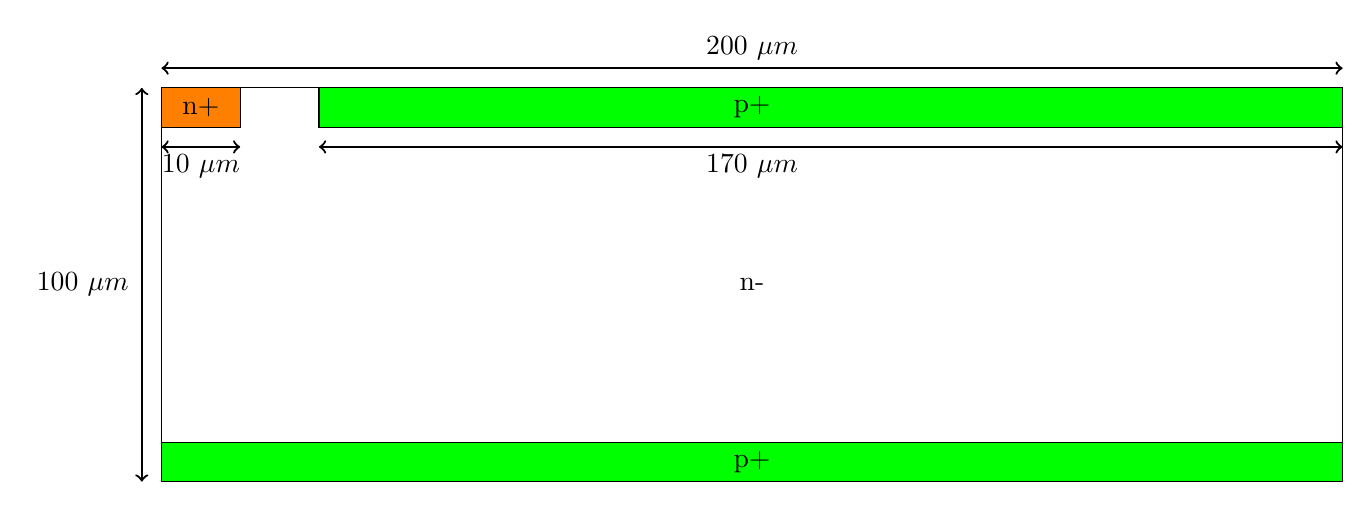
\begin{tikzpicture}
\def \thickness {5}
\def \width {15}
\draw [thick, <->] (-0.25,\thickness) -- (-0.25,0);
\draw [thick, <->] (0,\thickness+0.25) -- (\width,\thickness+0.25);
\draw [thick, <->] (2,\thickness-0.75) -- (\width,\thickness-0.75);
\node at (-1,0.5*\thickness) {100 $\mu m$};
\node at (0.5*\width,\thickness+0.5) {200 $\mu m$};
\node at (0.5*\width,\thickness-1) {170 $\mu m$};
\draw (0,0) rectangle (\width,\thickness);
\draw[fill=orange] (0,\thickness) rectangle (1,\thickness-0.5);
\draw [thick, <->] (0,\thickness-0.75) -- (1,\thickness-0.75);
\node at (0.5,\thickness-0.25) {n+};
\node at (0.5,\thickness-1) {10 $\mu m$};
\draw[fill=green] (2,\thickness-0.5) rectangle (\width,\thickness);
\node at (0.5*\width,\thickness-0.25) {p+};	
\draw[fill=green] (0,0) rectangle (\width,0.5);
\node at (0.5*\width,0.25) {p+};	
\node at (0.5*\width,0.5*\thickness) {n-};
\end{tikzpicture}
\caption{Input structure (SDD)}
\label{fig:SDD}
\end{figure}

\begin{figure}[h!]
     \centering
        \includegraphics[width=\textwidth]{equilibrium_potential_2d.png}
         \caption{Potential contour plot showing potential variation near the junction}
         \label{fig:pot_2d}
     \end{figure}

\begin{figure}[h!]
     \centering
        \includegraphics[width=\textwidth]{net_charge_equilibrium_2d.png}
         \caption{Accumulation of electrons producing negative charge near n+ region}
         \label{fig:pot_2d}
     \end{figure}

\subsection{Equilibrium potential and carrier density(1-D semiconductor p-n junction)}
Similarly, a $p+-n-n$ structure shown in \ref{fig:PIN} is solved here with similar doping profile. 
For an abrupt $p+-n$ junction \cite{bart}, depletion width is given by 
\begin{align*}
W_{dep} = \sqrt{\frac{2\epsilon_{Si} V_{bi}}{q N}} 
\end{align*}
where $N$ is the doping of lightly doped region.
For $N=10^{12}$, this is about $25 \mu m$. This is seen in the solved structure (see \ref{fig:pot_2d}) from $x=5 \mu m$ to about $x=30 \mu m$.

So, depletion width here should be about $25 \mu m$.

Built-in potential is given by 
\begin{align*}
V_{bi} \approx k_B T\ ln\left(\frac{N_A N_D}{n_i^2}\right)
\end{align*}

By above formula,it should be around 0.6 V for $p+-n$ which is seen in \ref{fig:pot_1d} at $x=10 \mu m$.

\begin{figure}[h!]
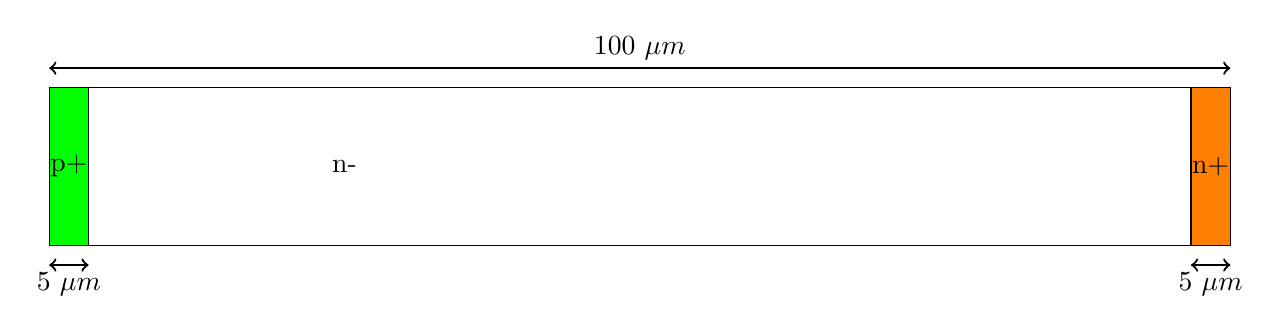
\begin{tikzpicture}
\def \thickness {2}
\def \width {15}
\draw [thick, <->] (0,\thickness+0.25) -- (\width,\thickness+0.25);
\draw [thick, <->] (0,-0.25) -- (0.5,-0.25);
\draw [thick, <->] (\width-0.5,-0.25) -- (\width,-0.25);
\node at (\width-0.25,-0.5) {5 $\mu m$};
\node at (0.25,-0.5) {5 $\mu m$};
\node at (0.5*\width,\thickness+0.5) {100 $\mu m$};
\draw (0,0) rectangle (\width,\thickness);
\draw[fill=green] (0,0) rectangle (0.5,\thickness);
\node at (0.25,0.5*\thickness) {p+};
\draw[fill=orange] (\width-0.5,0) rectangle (\width,\thickness);
\node at (\width-0.25,0.5*\thickness) {n+};
\node at (0.25*\width,0.5*\thickness) {n-};
\end{tikzpicture}
\caption{PIN diode}
\label{fig:PIN}
\end{figure}

\begin{figure}[h!]
     \centering
        \includegraphics[width=0.8\textwidth]{equilibrium_Potential_1d.png}
         \caption{Equilibrium Potential}
         \label{fig:pot_1d}	
     \end{figure}
     
\begin{figure}[h!]
     \centering
        \includegraphics[width=0.8\textwidth]{total_carriers_equilibrium.png}
         \caption{Carrier depletion near the $p+-n$ junction}
         \label{fig:car_1d}	
     \end{figure}     

\subsection{Potential and current density in a biased p-n junction}
In reverse bias, a potential barrier exists which blocks the flow of current while in forward bias, barrier lowers and large current flows. These features are visible in the following results.
 
\begin{figure}[h!]
     \centering
        \includegraphics[width=0.8\textwidth]{comparision_pin_fb.png}
         \caption{Potential barrier lowered in forward bias (compare with \ref{fig:pot_1d})}
         \label{fig:pot_fb}
     \end{figure}
     
\begin{figure}[h!]
     \centering
        \includegraphics[width=0.8\textwidth]{comparision_pin_rb.png}
         \caption{Potential barrier increased in reverse bias (compare with \ref{fig:pot_1d})}
         \label{fig:pot_fb}
     \end{figure}     

Current density for an ideal pn-junction diode \cite{bart} can be approximated by :
\begin{align*}
J = J_0 (e^{qV/k_BT}-1) 
\end{align*}


Current density for \ref{fig:PIN} is calculated.

\begin{figure}[h!]
     \centering
        \includegraphics[width=0.8\textwidth]{jv_diode_linear.png}
         \caption{Current density (Linear scale)}
         \label{fig:jv}
     \end{figure}

\begin{figure}[h!]
     \centering
        \includegraphics[width=0.8\textwidth]{jv_diode_log.png}
         \caption{Current density (Logarithmic scale) (compare with \ref{fig:jv_bart})}
		 \label{fig:jvl}     
     \end{figure}

\begin{figure}[h!]
     \centering
        \includegraphics[width=0.8\textwidth]{bart.png}
         \caption{Image taken from \cite{bart}}
		 \label{fig:jv_bart}     
     \end{figure}

In forward bias, current becomes very high when $V>=V_{bi}$. Here, $V_{bi} = 0.6\ V$. In reverse bias, very low current flows (see  \ref{fig:jv}). Also, exponential relationship can be seen as J-V plot is linear in logarithmic scale in forward bias as seen in \ref{fig:jvl}.
